\documentclass{article}
\usepackage[utf8]{inputenc}
\usepackage{graphicx}

% change reference style to [1], remove stupid sorting, language changed so date in ddmmyyyy
\usepackage[backend=biber, style=numeric, sorting=none, language=australian]{biblatex}
\addbibresource{References.bib}

\title{Dissertation - Detecting User Engagement Using Mouse Tracking Data}
\author{David Saunders (910995)}
\date{September 2020}

\begin{document}
\maketitle

\begin{abstract} 
    Write abstract here
\end{abstract}

\tableofcontents

% Toms layout

% Motivation
% Related Work
% Implementation
% Results
% Conclusion

\section{Motivation}

% Why is it important
% Why is it a hard problem/problems
% Why other authors have failed
% My contributions are - bullet list
% My idea to fix it

Detecting use engagement is an important science across multiple disciplines.

It is a hard problem because, among other things I will touch on, it is hard to quantify exactly what user engagement is exactly.
One author defined it as 'XYZ' [look at my previous work for references].

However the previous authors have failed to detect and measure user engagement as X,Y,Z.

\subsection{Contributions}
% The contributions are 1,2,3 (everyone likes 3s)
% Take aways of how it will help them.

In this project my contributions to fix it are, -a system to classify users, a way of visualising their mouse paths, ways to directly and quantitatively compare different users, and a multistage semi-supervised based binary classification output to answer the question of 'are users engaged'.

\section{Related Work}

% Convince the reader you've done enough work and research in the area.
% Convince them it was hard and the topic is hard so you need to help.
% You've tried other peoples techniques.

All related work about actual other attempts to detect user engagement from mouse tracking data.
Other subsections will be like miniature literature reviews or something?

\subsection{Semi Supervised Learning}
This will be a key aspect of the project as we only have definitive labels for part of our data.
This reflects the challenges of real world data, by some estimates only 2\% (made up number) of all data is structured and labelled, the rest is unstructured [find reference].

% Do a literature review type of thing where I review semi supervised learning, talk about methods and how they can be applied to what I'm trying to do.

\subsection{N-Grams}
This paper has a nice scientific explanation of n-grams \cite{tomovic2006n}.
Either cite this paper or more likely look at their reference for n-grams and cite that.

\subsection{Hidden Markov Models}

% explanation from scratch: https://towardsdatascience.com/hidden-markov-model-implemented-from-scratch-72865bda430e

Paper Tom send me about HMM for text classification that I might be able to use \cite{collins2016tagging}.

Paper claims to use HMM for spam detection, I think they actually just use it to detect misspellings of words or something which is used by spam to hide from filters \cite{gordillo2007hmm}.
Probably could find a better spam detecting HMM, I just like how this almost does something different from the title, which my diss will end up doing.

This paper was recommended by someone on stack overflow as an old influential paper in the field with tens of thousands of references \cite{rabiner1989tutorial}.
Called a tutorial on HMM and its so old so original source. 
Would definitely be good to reference if I include any of the mathematics behind HMMs. 

Someone's dissertation on the topic of generating synthetic data with HMMs.
This can be a good way to create synthetic data \cite{ferrando2018generating}.

Maybe this would belong under implementation?
%HMM-Example-Diagram.png
\begin{figure}[ht]
    \centering
    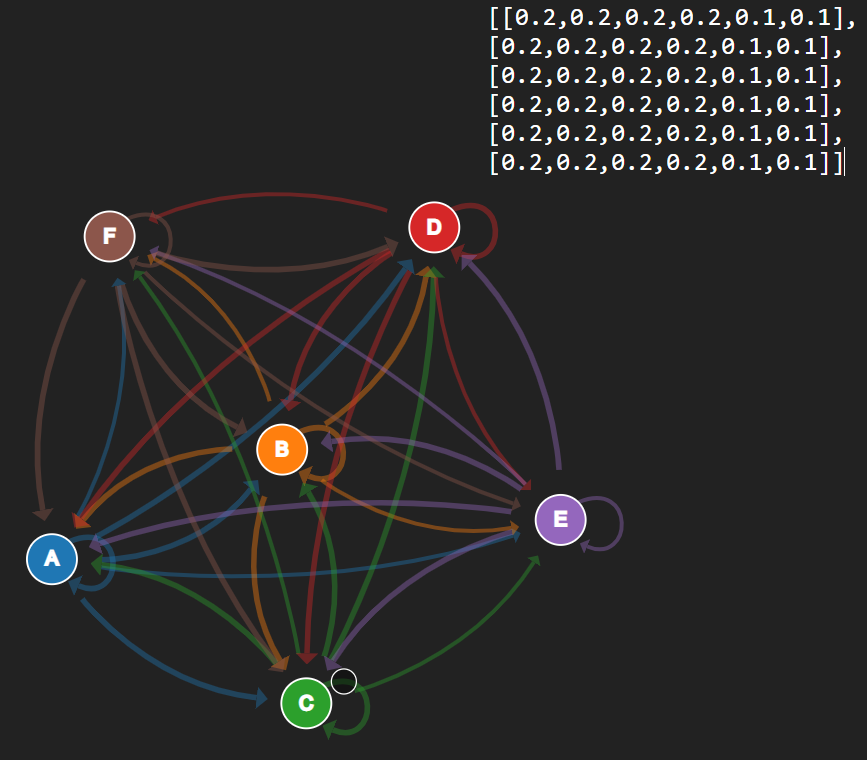
\includegraphics[scale=0.55]{HMM-Example-Diagram.png}
    \caption{Diagram of a Markov Chain model representing a users mouse position}
    \label{fig:Markov}
\end{figure}

Figure \ref{fig:Markov} shows the states of a markov model of my system with states A-E representing sliders 1-5 and state F representing an html element.
In the top right we can see a possible transition matrix of our system.

\section{Implementation}

% Talk about all different steps you took?

\section{Data Pipeline}

When planning and completing this project many decisions were made about the steps taken to convert the raw data to a finished product/classification.
This section may act as an overview of the project, detailing the different sections of work, what they may contain, and the order in which they will be completed.

\begin{figure}[ht]
    \centering
    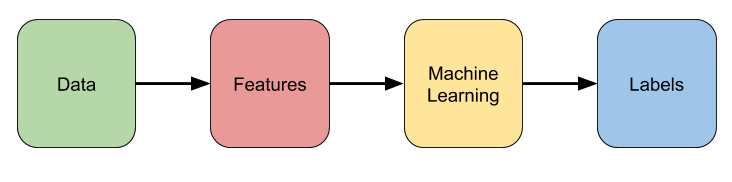
\includegraphics[scale=0.55]{Images/Data-Pipeline.png}
    \caption{Diagram of the Data Pipeline of the project.}
    \label{fig:test}
\end{figure}

% Everyone is a question

\subsection{Data}

% Duplicate or remove to deal with imbalances.
% Probably less effective focusing on this rather than features.

Here I will summarise what I have done to the data.
As previously mentioned the data was gathered through a lab study and an online study.
The purpose of the online study was to gather a larger amount of data that was possible to do so in person.
The aim of this was to make any results more statically significant.
Data was recorded in a big JSON dump with lots of irrelevant and repealed data relating to the users background and not their mouse movements.
Pythons JSON couldn't directly convert the data as mouse events were stored as a nested JSON dictionary and there were errors in the way it was written making it invalid JSON.
Took ages and should explain more indepth, but then finally got data into a tabular data format of a csv which I am more comfortable working with.
Ended up with over 100,000 lines? Might have been more. 

This leads to the problem of imbalanced data samples.
There were approximately 11 lab data and 400 online data, meaning that there were 40x as many data samples from one class compared to the other.
As stated in my assumptions, we can say that the lab participants were paying attention, where as the online participants may or may not have been paying attention.

If the classes were balanced then simple approach may be to treat this problem as binary classification problem.
Using something like a Support Vector Machine we could classify a given point as lab or online / paying attention or possibly paying attention based on their proximity to other data points.
To do so we would need to have balanced classes otherwise the algorithm would have a high accuracy from just classifying everything as possibly paying attention as that is the most frequent class.
There are two main methods of dealing with class imbalances, removing data samples and creating new data samples.

It was decided that creating new data samples would be best as there is not a whole lot of data to work with, so there would be a strong preference to keep the data we have.
New points can be created by sampling from a distribution (reference) but here it was decided just to duplicate the samples as there was no discernible distribution of the data.
Another method is to copy the points, altering them slightly, this was considered but not used in the end.
Each lab study data sample was copied 40 times to even out the classes.

\subsection{Features}

% Tom said something about this being where I should spend the most time of my project.
% Spending time here will be more time effective than other sections.
% This is what people wanna see?
% Evaluating effectiveness of different features.

% What do I so to the raw data.

% What are good features? Big/Good question split into smaller sections.

This part of the pipeline refers to what features I am going to extract from the data.
Features of data can be defined as 'attributes or interesting things from the data'. [reference]
These will consist of both raw and created features, but what do I mean by this?
Raw features will consist of the the number of mouse events recorded, while a created feature could be comparing the trace of users cursor data when using the program.

\subsection{Machine Learning}

% What ML will I do and what algorithm.
% MAybe clustering algorithm but on what data?

Once we have insightful features from the data we can consider what machine learning algorithm would be most appropriate to use on the data.
This will obviously be highly dependent on what form the final features are in.
For example if the features are numerical values such as time taken to complete task and number of mouse events then an algorithm such as a Support Vector Machine would be a good choice.
If the data is in the form of sequential data such as a list of all mouse events then something like a LSTM or RNN network would be best suited.
If the features output was an image such as a trace of mouse position over time then a CNN could be a good choice as they're designed for image data.
It is likely that text classification algorithms will be used when comparing the targets of mouse events.
Comparing n-grams can be done with algorithms such as XYZ [reference].
Other text classification algorithms such as cosine similarity or sentiment analysis could also be used.


\subsection{Labels}

% Who's paying attention

Lastly an important section of the pipeline, as it reflects the final outputs of the system.
Labels will refer to which users are classified as paying attention and which users are not.
A key aspect of this project will be semi-supervised learning.
That is we have some data points we can confirm were paying attention, and others where they're level of attention was questionable.
Once we have an algorithm that can classify some users as paying attention or not we can rerun the algorithm with these preliminary outputs as new training data.
If this is done recursively then we can end up with a system that can split all data points into the 2 classes, perhaps with a degree of confidence given as a percentage.

\section{Results}

% talk about results

\subsection{Table or graph of results}

\section{Conclusion}



\printbibliography

\end{document}